\section{الگوریتم \lr{SAC}}
\label{sec:sac_results}

الگوریتم \lr{SAC}  از روش‌های نوین یادگیری تقویتی است که با استفاده از مفهوم آنتروپی، تعادل بهتری بین اکتشاف و بهره‌برداری ایجاد می‌کند. این الگوریتم در شرایط فضاهای پیوسته عملکرد قابل توجهی دارد.

\begin{figure}[H]
	\centering
	
	% سطر اول
	\subfloat[\lr{SAC} استاندارد]{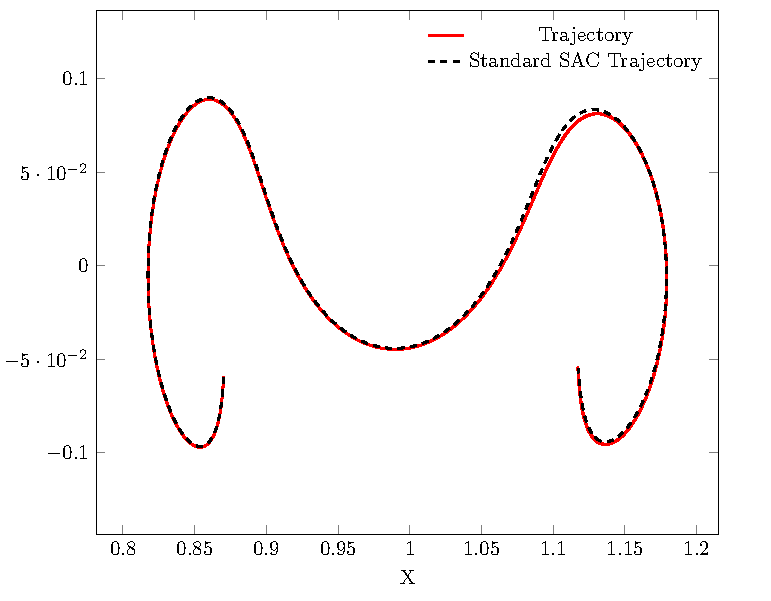
\includegraphics[width=.45\textwidth]{plots/sac/trajectory_force/plot_trajectory.pdf}}%
	\subfloat[\lr{SAC} بازی مجموع‌صفر]{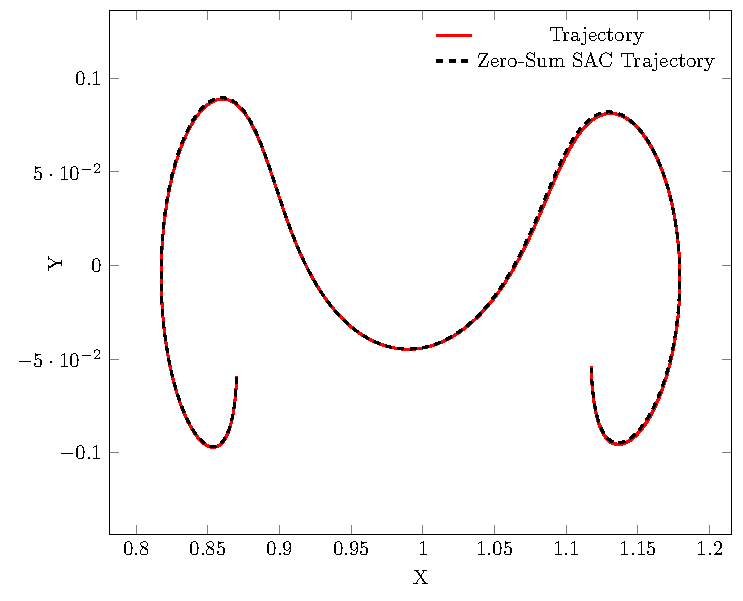
\includegraphics[width=.45\textwidth]{plots/sac/trajectory_force/plot_trajectory_zs.pdf}}%
	
	\caption{مسیر طی‌شده فضاپیما با \lr{SAC} استاندارد و نسخه بازی مجموع‌صفر \lr{MA-SAC}.}
\end{figure}


\begin{figure}[H]
	\centering
	
	% سطر اول
	\subfloat[\lr{SAC} استاندارد]{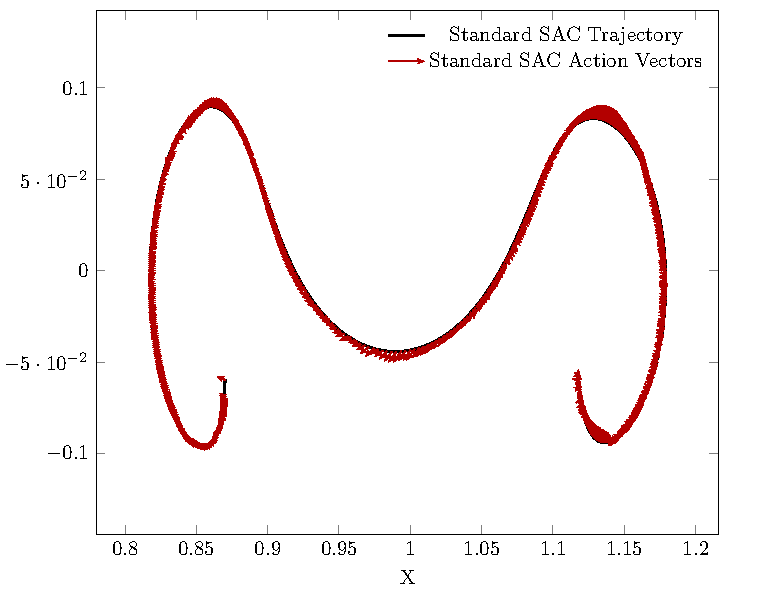
\includegraphics[width=.45\textwidth]{plots/sac/trajectory_force/plot_trajectory_force.pdf}}%
	\subfloat[\lr{SAC} بازی مجموع‌صفر]{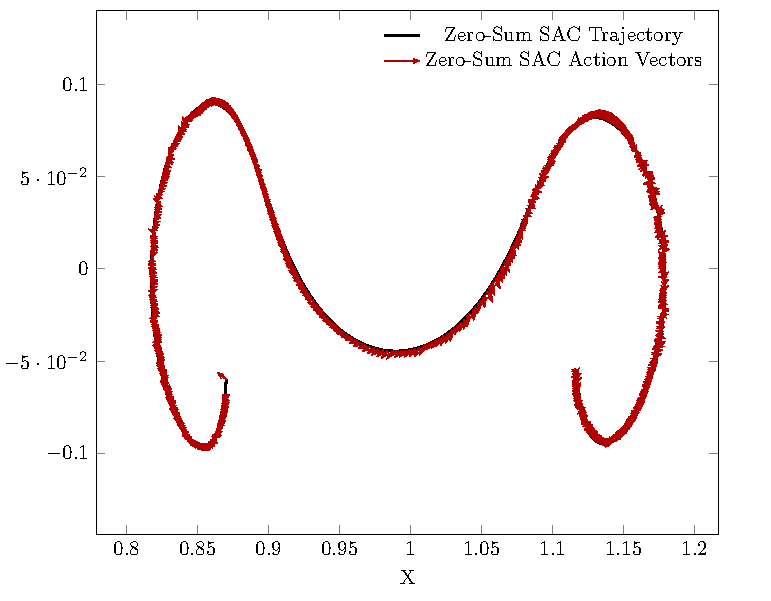
\includegraphics[width=.45\textwidth]{plots/sac/trajectory_force/plot_trajectory_force_zs.pdf}}%
	
	\caption{مسیر و فرمان پیشران فضاپیما در \lr{SAC} استاندارد و نسخه بازی مجموع‌صفر \lr{MA-SAC}.}
\end{figure}

الگوریتم \lr{SAC} در هر دو حالت عملکرد قابل قبولی ارائه می‌دهد. ویژگی خاص این الگوریتم در تنظیم خودکار پارامتر آنتروپی باعث می‌شود که بتواند تعادل مناسبی بین اکتشاف و بهره‌برداری ایجاد کند، اما نسخه بازی مجموع‌صفر آن در شرایط سخت‌تر مقاومت بیشتری نشان می‌دهد.





\begin{table}[H]
	\centering
	\setlength{\tabcolsep}{3pt}
	\small
	\begin{tabular}{@{} R{3.2cm} *{8}{C{1.05cm}} @{}}
		\toprule
		\multirow{2}{*}{\makecell[r]{سناریو}}
		& \multicolumn{2}{c}{پاداش تجمعی} & \multicolumn{2}{c}{مجموع خطای مسیر}
		& \multicolumn{2}{c}{مجموع تلاش کنترلی} & \multicolumn{2}{c}{احتمال شکست} \\
		\cmidrule(lr){2-3}\cmidrule(lr){4-5}\cmidrule(lr){6-7}\cmidrule(lr){8-9}
		& {\rotatebox[origin=c]{90}{\lr{SAC}}} & {\rotatebox[origin=c]{90}{\lr{MA-SAC}}}
		& {\rotatebox[origin=c]{90}{\lr{SAC}}} & {\rotatebox[origin=c]{90}{\lr{MA-SAC}}}
		& {\rotatebox[origin=c]{90}{\lr{SAC}}} & {\rotatebox[origin=c]{90}{\lr{MA-SAC}}}
		& {\rotatebox[origin=c]{90}{\lr{SAC}}} & {\rotatebox[origin=c]{90}{\lr{MA-SAC}}} \\
		\midrule
		شرایط اولیه تصادفی
		&
		$-4.69$ & ${-2.98}$ & $0.29$ & ${0.26}$ & $1.37$ & $1.37$ & $1.00$ & $1.00$ \\
		اغتشاش در عملگرها
		&
		$-1.95$ & ${-1.93}$ & $8.02$ & ${7.72}$ & $3.09$ & $3.09$ & $1.00$ & $1.00$ \\
		عدم تطابق مدل
		&
		$-4.89$ & ${-4.35}$ & $0.38$ & ${0.26}$ & $1.16$ & $1.16$ & $1.00$ & $1.00$ \\
		مشاهده ناقص
		&
		$-3.63$ & ${-0.44}$ & $1.95$ & ${0.07}$ & $1.99$ & $1.99$ & $1.00$ & ${0.00}$ \\
		نویز حسگر
		&
		$-0.89$ & ${0.12}$ & $0.12$ & $0.12$ & $1.86$ & $1.86$ & $0.00$ & $0.00$ \\
		تأخیر زمانی
		&
		$-4.14$ & ${-0.05}$ & $1.87$ & ${0.01}$ & $1.25$ & $1.25$ & $1.00$ & ${0.00}$ \\
		\bottomrule
	\end{tabular}
	\caption{مقایسه عملکرد \lr{SAC} و \lr{MA-SAC} در سناریوهای مختلف مقاومت}
	\label{tab:sac_comparison}
\end{table}